\documentclass[review,3p]{elsarticle}

% --- Packages ---
\usepackage{lineno}
\usepackage{hyperref}
\usepackage{booktabs}
\usepackage{amsmath}
\usepackage{amssymb}
\usepackage{graphicx}
\usepackage{listings}
\usepackage{xcolor}
\usepackage{algorithm}
\usepackage{algpseudocode}
\usepackage{multirow}
\usepackage{nomencl}
\usepackage{url}
\usepackage{siunitx}
\usepackage{tikz}
\usetikzlibrary{shapes.geometric, arrows.meta, positioning}

% Line numbers for review
\linenumbers

% Nomenclature
\makenomenclature

% Listings style for EES code
\definecolor{eescomment}{rgb}{0.0,0.5,0.0}
\definecolor{eesstring}{rgb}{0.58,0.0,0.82}
\definecolor{eeskeyword}{rgb}{0.0,0.0,0.8}
\lstdefinelanguage{EES}{
  morekeywords={FUNCTION,PROCEDURE,END,CALL,IF,THEN,ELSE,ENDIF,REPEAT,UNTIL,GOTO},
  sensitive=false,
  morecomment=[s]{"}{"},
  morecomment=[s]{\{}{\}},
  morecomment=[l]{//},
  morestring=[b]',
}
\lstset{
  language=EES,
  basicstyle=\ttfamily\small,
  keywordstyle=\color{eeskeyword}\bfseries,
  commentstyle=\color{eescomment}\itshape,
  stringstyle=\color{eesstring},
  numbers=left,
  numberstyle=\tiny\color{gray},
  numbersep=5pt,
  frame=single,
  breaklines=true,
  captionpos=b,
  xleftmargin=15pt,
  framexleftmargin=15pt,
}

\journal{Applied Thermal Engineering}

\begin{document}

\begin{frontmatter}

% --- Title ---
\title{CoolSolve: An Open-Source Equation Solver with Integrated Thermodynamic Properties}

% --- Author ---
\author[uliege]{Sylvain Quoilin\corref{cor1}}
\ead{squoilin@uliege.be}
\cortext[cor1]{Corresponding author}
\address[uliege]{Thermodynamics Laboratory, Faculty of Applied Sciences,
  All\'ee de la D\'ecouverte 17, 4000 Li\`ege, Belgium}

% --- Highlights ---
% Required by Applied Thermal Engineering (3-5 bullet points, max 85 chars each)
% Highlights are submitted as a separate file in the Elsevier submission system.
% They are listed here for reference:
% - Open-source equation solver compatible with the EES modeling language
% - Six nonlinear solvers with configurable pipeline and parallel execution
% - CoolProp integration for thermodynamic properties with analytical derivatives
% - Structural analysis via Hopcroft-Karp matching and Tarjan decomposition
% - Web-based GUI with real-time solving, parametric studies, and diagrams

% --- Abstract ---
\begin{abstract}
This paper presents CoolSolve, an open-source equation solver designed for thermodynamic system modeling. CoolSolve parses an equation-based modeling language compatible with the syntax of Engineering Equation Solver (EES), a widely used commercial tool for teaching and research in thermal engineering. Unlike EES, CoolSolve is open-source, cross-platform, and integrates the open-source CoolProp library for thermodynamic property calculations. The solver features a configurable pipeline of six numerical algorithms---Newton with non-monotone line search, Trust-Region Dogleg, Levenberg-Marquardt, N-dimensional bisection, homotopy continuation, and partitioned block updates---which can be executed sequentially or in parallel (first-to-converge wins). A structural analysis layer based on the Hopcroft-Karp matching algorithm and Tarjan's strongly connected components decomposition automatically decomposes equation systems into solvable blocks. Forward-mode automatic differentiation provides exact Jacobians without finite differences. CoolSolve further integrates CoolProp's low-level API with analytical derivatives and thread-local caching for performance. A web-based graphical user interface enables browser-based modeling with real-time solving, parametric studies, and interactive thermodynamic diagrams. The solver is validated on 40 thermodynamic models covering Rankine cycles, organic Rankine cycles, heat pumps, compressors, and heat exchangers, achieving a 92\% solve rate with the default pipeline. All code is released under the MIT license, and an online instance is publicly available for immediate use.
\end{abstract}

% --- Keywords ---
% Required by Applied Thermal Engineering (max 6 keywords)
\begin{keyword}
equation solver \sep thermodynamic modeling \sep open-source software \sep CoolProp \sep nonlinear systems \sep organic Rankine cycle
\end{keyword}

\end{frontmatter}

% ===================================================================
% NOMENCLATURE
% ===================================================================
\section*{Nomenclature}
\begin{tabular}{@{}ll@{}}
\toprule
\textbf{Symbol} & \textbf{Description} \\
\midrule
$\mathbf{F}(\mathbf{x})$ & Residual vector \\
$\mathbf{J}$    & Jacobian matrix \\
$\mathbf{x}$    & Vector of unknown variables \\
$\Delta\mathbf{x}$ & Newton step \\
$\lambda$       & Levenberg-Marquardt damping parameter \\
$\Delta$        & Trust-region radius \\
$\phi$          & Merit function, $\phi = \frac{1}{2}\|\mathbf{F}\|^2$ \\
$\rho$          & Gain ratio (actual vs.\ predicted reduction) \\
$M$             & Non-monotone memory parameter \\
$n$             & Number of unknowns in a block \\
\midrule
\textbf{Abbreviation} & \\
\midrule
AD    & Automatic differentiation \\
BLT   & Block lower triangular \\
EES   & Engineering Equation Solver \\
FD    & Finite differences \\
GUI   & Graphical user interface \\
HVAC  & Heating, ventilation, and air conditioning \\
LM    & Levenberg-Marquardt \\
ORC   & Organic Rankine Cycle \\
SCC   & Strongly connected component \\
SPA   & Single-page application \\
SSE   & Server-Sent Events \\
VLE   & Vapor-liquid equilibrium \\
\bottomrule
\end{tabular}

% ===================================================================
\section{Introduction}
\label{sec:introduction}
% ===================================================================

Thermodynamic modeling is essential for the design, optimization, and operation of energy conversion systems such as power plants, refrigeration systems, heat pumps, and organic Rankine cycles (ORCs) \cite{Quoilin2013, Lecompte2015}. These models typically consist of systems of nonlinear algebraic equations that couple mass and energy balances with thermodynamic property calculations. Solving such systems requires both a robust numerical solver and access to accurate thermodynamic data for working fluids.

Engineering Equation Solver (EES), developed by F-Chart Software \cite{Klein2023, EES2024}, has been the dominant tool in this domain for over three decades. EES provides an intuitive equation-based modeling language in which users write equations in any order, and the solver automatically identifies unknowns and determines the solution. Its tight integration with built-in thermodynamic property data for hundreds of fluids has made EES the standard tool for teaching thermodynamics and thermal system design in universities worldwide \cite{Nellis2016}. Research groups have used EES extensively to develop and validate models of ORCs \cite{Quoilin2011, Lemort2009}, heat exchangers \cite{Desideri2014}, compressors, and other thermal components.

Despite its widespread adoption, EES has significant limitations that hinder modern engineering workflows:
\begin{itemize}
    \item \textbf{Closed-source and proprietary}: the source code is not available, preventing independent verification, customization, or extension of the solver algorithms.
    \item \textbf{Platform restriction}: EES runs only on Microsoft Windows, excluding users on Linux and macOS.
    \item \textbf{License cost}: commercial licenses are expensive, creating barriers for students, researchers in developing countries, and open-science initiatives.
    \item \textbf{Reproducibility}: models cannot be freely shared with all collaborators, and solver behavior cannot be independently audited---a fundamental problem for scientific reproducibility.
    \item \textbf{Legacy architecture}: EES uses a single solver (Newton's method with modifications), with limited options for configuring solver behavior or adding new algorithms.
\end{itemize}

The importance of open-source tools and open data for energy research has been articulated forcefully by Pfenninger et al.\ \cite{Pfenninger2017, Pfenninger2018}, who argue that closed, proprietary models create ``black boxes'' that undermine scientific credibility and slow down innovation. They call for the energy modeling community to adopt open-source practices to ensure transparency, reproducibility, and collaborative development.

In the thermodynamic property domain, the CoolProp library \cite{Bell2014} has demonstrated the viability of the open-source approach. CoolProp provides thermophysical properties for over 120 pure and pseudo-pure fluids based on high-accuracy Helmholtz energy equations of state, as well as mixture properties and incompressible fluids. It is written in C++ with wrappers for Python, MATLAB, and other languages, and has been cited thousands of times in the scientific literature.

However, to date there has been no open-source equation solver that combines (i)~compatibility with the EES modeling language, (ii)~integration with CoolProp thermodynamic properties, and (iii)~a modern multi-algorithm solver architecture. Several alternative tools exist in adjacent domains:
\begin{itemize}
    \item \textbf{Modelica}-based environments (OpenModelica, Dymola) \cite{Modelica2023, Wetter2014} provide powerful equation-based modeling, but use a fundamentally different language oriented toward dynamic simulation with differential-algebraic equations. The learning curve is steep, and the ecosystem is optimized for transient simulation rather than steady-state thermodynamic design.
    \item General-purpose mathematical solvers (MATLAB \texttt{fsolve}, SciPy \texttt{fsolve}, Julia \texttt{NLsolve.jl}) can solve nonlinear systems but require users to manually formulate the problem in procedural code, manage thermodynamic property calls, and configure solver options---losing the declarative, equation-based workflow that makes EES accessible.
    \item \textbf{REFPROP} \cite{Wagner2002} provides high-accuracy thermodynamic properties but is also commercial, closed-source, and does not include an equation solver.
\end{itemize}

This paper presents CoolSolve, an open-source equation solver that addresses these gaps. CoolSolve parses a modeling language compatible with the EES syntax, making it possible to run existing EES models with minimal modification. It integrates CoolProp for thermodynamic properties, runs on all major platforms (Linux, macOS, Windows), and introduces a novel configurable solver pipeline with six complementary algorithms that can be executed in parallel. The solver architecture incorporates structural analysis, forward-mode automatic differentiation, and symbolic block reduction as key innovations beyond the capabilities of EES.

The main contributions of this work are:
\begin{enumerate}
    \item An open-source, cross-platform equation solver compatible with the EES modeling language, integrating CoolProp thermodynamic properties.
    \item A configurable solver pipeline with six algorithms---Newton with non-monotone line search, Trust-Region Dogleg, Levenberg-Marquardt, N-dimensional bisection, homotopy continuation, and partitioned block updates---with sequential and parallel execution modes.
    \item Structural analysis via Hopcroft-Karp matching and Tarjan's decomposition, combined with symbolic block reduction and automatic re-decomposition.
    \item Validation on 40 thermodynamic models demonstrating robustness across different system types and solver configurations.
    \item A web-based GUI enabling browser-based modeling, solving, parametric studies, and interactive thermodynamic diagrams, deployable locally or online.
\end{enumerate}

The remainder of this paper is organized as follows. Section~\ref{sec:language} describes the EES-compatible modeling language. Section~\ref{sec:structural} presents the structural analysis algorithms. Section~\ref{sec:solvers} details the solver pipeline and individual algorithms. Section~\ref{sec:coolprop} discusses the CoolProp integration strategy. Section~\ref{sec:gui} describes the web-based GUI. Section~\ref{sec:validation} presents the validation results. Section~\ref{sec:conclusion} concludes the paper.

% ===================================================================
\section{The EES-Compatible Modeling Language}
\label{sec:language}
% ===================================================================

CoolSolve implements a parser for a modeling language that is syntactically compatible with the Engineering Equation Solver (EES) language \cite{Klein2023}. This design choice is deliberate: the EES language has been used for decades in university courses and research publications, and a large body of existing models is written in this language. By supporting the same syntax, CoolSolve enables users to transition existing models with minimal effort and eliminates the need to learn a new language.

\subsection{Language Features}

The EES language is equation-based: users write equations in any order, and the solver determines which variables are unknowns and in what order to solve them. This declarative approach is particularly intuitive for engineering problems where equations come directly from textbook formulations. The main language features supported by CoolSolve are:

\begin{itemize}
    \item \textbf{Equations}: written with the \texttt{=} operator expressing equality (not assignment). Variables can appear on either side.
    \item \textbf{Thermodynamic function calls}: calls such as \texttt{enthalpy(R134a, T=300, P=1E5)} use named arguments to specify the fluid, input properties, and their values. This syntax naturally maps to CoolProp property queries.
    \item \textbf{Variables}: scalar variables and array variables (e.g., \texttt{T[1]}, \texttt{h[2]}). Variable names are case-insensitive.
    \item \textbf{Procedures and functions}: \texttt{FUNCTION} and \texttt{PROCEDURE} blocks with local scoping, supporting procedural statements (\texttt{:=} assignment), conditional logic (\texttt{IF-THEN-ELSE}), and the \texttt{CALL} syntax for procedure invocation.
    \item \textbf{Comments}: three comment styles (\texttt{"..."} for visible comments, \texttt{\{...\}} for invisible comments, \texttt{//} for line comments).
    \item \textbf{Unit annotations}: strings like \texttt{"[kJ/kg]"} following a value to document units.
    \item \textbf{Directives}: preprocessor-like directives (\texttt{\$ifnot}, \texttt{\$endif}) for conditional compilation.
\end{itemize}

Listing~\ref{lst:example} shows a simple refrigeration cycle model written in the EES-compatible language.

\begin{lstlisting}[caption={Simple refrigeration cycle model in the EES-compatible language.},label={lst:example},float=tp]
"Simple vapor compression refrigeration cycle"
T_ev = -10          "Evaporator temperature [C]"
T_cd = 30           "Condenser temperature [C]"
eta_s = 0.8         "Isentropic efficiency [-]"
Q_dot_ev = 50000    "Cooling capacity [W]"

"Saturation pressures"
P_ev = pressure(R134a, T=T_ev, x=0.5)
P_cd = pressure(R134a, T=T_cd, x=0.5)

"Cycle state points"
h_1 = enthalpy(R134a, T=T_ev, x=1)
s_1 = entropy(R134a, T=T_ev, x=1)
h_2s = enthalpy(R134a, P=P_cd, s=s_1)
h_2 = h_1 + (h_2s - h_1) / eta_s
h_3 = enthalpy(R134a, T=T_cd, x=0)
h_4 = h_3

"Energy balances"
M_dot = Q_dot_ev / (h_1 - h_4)
W_dot = M_dot * (h_2 - h_1)
COP = Q_dot_ev / W_dot
\end{lstlisting}

\subsection{Parsing and IR Construction}

CoolSolve uses a Parsing Expression Grammar (PEG) parser implemented with the cpp-peglib library. The parser produces an Abstract Syntax Tree (AST) that is then transformed into an Intermediate Representation (IR). The IR extracts:
\begin{itemize}
    \item The set of variables appearing in each equation.
    \item The incidence matrix relating equations to variables.
    \item Thermodynamic function calls with their fluid name, property type, and named arguments.
    \item Procedure and function definitions with their local scoping rules.
\end{itemize}

The IR is the foundation for all subsequent analysis: structural decomposition, automatic differentiation, and numerical evaluation.

% ===================================================================
\section{Structural Analysis}
\label{sec:structural}
% ===================================================================

Before solving, CoolSolve performs a structural analysis of the equation system to decompose it into smaller blocks that can be solved independently and sequentially. This decomposition is critical for efficiency and robustness: solving many small subsystems is far easier than solving one large monolithic system.

\subsection{Bipartite Matching: Hopcroft-Karp Algorithm}

The first step is to find a maximum bipartite matching between equations and variables. Each equation is matched to one ``output'' variable that it will determine. CoolSolve implements the Hopcroft-Karp algorithm \cite{HopcroftKarp1973}, which finds a maximum matching in $O(E\sqrt{V})$ time, where $E$ is the number of edges in the incidence graph and $V$ is the number of vertices.

This matching defines a direction for each equation: the matched variable is the one ``solved for'' by that equation, while the remaining variables are inputs. If the maximum matching is smaller than the number of equations, the system is structurally singular (over- or under-determined), and CoolSolve reports a diagnostic error before attempting to solve.

\subsection{Block Decomposition: Tarjan's Algorithm}

Given the matching, a directed dependency graph is constructed: equation $i$ depends on equation $j$ if the output variable of $j$ appears as an input in $i$. Tarjan's algorithm \cite{Tarjan1972} identifies the strongly connected components (SCCs) of this directed graph. Each SCC corresponds to a group of equations that are mutually coupled and must be solved simultaneously---an \emph{algebraic loop}.

The SCCs are then topologically sorted to produce a Block Lower Triangular (BLT) form. This ordering guarantees that when solving block $k$, all variables from blocks $1, \ldots, k-1$ are already known. The result is a sequence of independent blocks, each of which is a small nonlinear system (or a single explicit equation).

\subsection{Symbolic Block Reduction}

CoolSolve optionally performs symbolic preprocessing to further reduce block sizes before numerical solving. When enabled (\texttt{enableSymbolicReduction} option), three techniques are applied iteratively until a fixed point:
\begin{enumerate}
    \item \textbf{CoolProp call inversion}: if an equation computes a thermodynamic property as the block's matched output (e.g., $h = \text{enthalpy}(\text{R134a}, T{=}T, P{=}P)$) and one of the named-argument inputs is the only block unknown, the call is symbolically inverted (e.g., $T = \text{temperature}(\text{R134a}, H{=}h, P{=}P)$).
    \item \textbf{Explicit extraction}: equations where all variables except the matched output are already known are evaluated directly, removing their output from the unknown set.
    \item \textbf{Equation substitution}: variables that appear in no other block equation after extraction are eliminated along with their defining equation.
\end{enumerate}

After reduction, a \textbf{post-reduction re-decomposition} is performed by running Tarjan's algorithm on the reduced dependency graph. This can split a large monolithic block into several independent sub-blocks, dramatically reducing the computational cost (Newton's method cost scales as $O(n^3)$ per iteration due to the linear solve).

% ===================================================================
\section{Solver Pipeline}
\label{sec:solvers}
% ===================================================================

A key innovation in CoolSolve is the configurable solver pipeline. Rather than relying on a single algorithm, CoolSolve provides six complementary solvers that address different failure modes of nonlinear equation solving. The pipeline is user-configurable and can operate in two modes:
\begin{itemize}
    \item \textbf{Sequential mode} (default): solvers are tried in order; if one fails, the next is attempted with the best state reached so far.
    \item \textbf{Parallel mode}: all solvers are launched simultaneously in separate threads using \texttt{std::async}; the first to converge wins, and a shared cancellation token stops the others.
\end{itemize}

The default pipeline order is: Newton $\rightarrow$ Trust-Region $\rightarrow$ Levenberg-Marquardt $\rightarrow$ BisectionND $\rightarrow$ Homotopy $\rightarrow$ Partitioned. This ordering reflects increasing robustness at the cost of decreasing efficiency.

The pipeline is configurable via a plain-text configuration file (\texttt{coolsolve.conf}) placed alongside the model file. Users can select which solvers to include, set their order, and tune individual solver parameters.

\subsection{Newton's Method with Non-Monotone Line Search}

The primary solver is Newton's method, which at each iteration solves the linear system:
\begin{equation}
    \mathbf{J}(\mathbf{x}_k) \, \Delta\mathbf{x}_k = -\mathbf{F}(\mathbf{x}_k)
\end{equation}
where $\mathbf{J}$ is the Jacobian matrix and $\mathbf{F}$ is the residual vector. The step $\Delta\mathbf{x}_k$ is subjected to a backtracking line search.

CoolSolve implements the non-monotone line search of Grippo, Lampariello, and Lucidi \cite{Grippo1986}. Instead of requiring the merit function $\phi(\mathbf{x}) = \frac{1}{2}\|\mathbf{F}(\mathbf{x})\|^2$ to decrease at every step (monotone Armijo condition), the non-monotone variant compares against the maximum over the last $M$ iterations:
\begin{equation}
    \phi(\mathbf{x}_k + \alpha \, \Delta\mathbf{x}_k) \leq \max_{0 \leq j \leq \min(k,M-1)} \phi(\mathbf{x}_{k-j}) + c \, \alpha \, \nabla\phi_k^T \Delta\mathbf{x}_k
    \label{eq:nonmonotone}
\end{equation}
where $c$ is the Armijo parameter (default $10^{-4}$) and $M$ is the memory parameter (default 10). To prevent the reference from becoming arbitrarily large due to a single bad iterate, the reference is capped at $\min(\max(\text{history}), R \cdot \phi_k)$ with $R=10$.

This non-monotone strategy allows the solver to temporarily accept steps that increase the merit function, helping it escape narrow curved valleys and saddle points that trap monotone methods.

The Newton solver also supports \textbf{Broyden quasi-Newton updates} \cite{Broyden1965}: when the \texttt{broydenRecomputeInterval} is set to $K > 0$, a full Jacobian is computed every $K$ iterations, with rank-1 Broyden updates in between. This significantly reduces the number of expensive thermodynamic property evaluations for large blocks.

\subsection{Trust-Region Dogleg Method}

The Trust-Region Dogleg method \cite{Nocedal2006} maintains a trust radius $\Delta$ and computes a \emph{dogleg step} that blends the steepest-descent direction with the Newton direction:
\begin{equation}
    \mathbf{d}_{\text{dogleg}} = \begin{cases}
        \mathbf{d}_N & \text{if } \|\mathbf{d}_N\| \leq \Delta \\
        \tau \, \mathbf{d}_C & \text{if } \|\mathbf{d}_C\| \geq \Delta \\
        \mathbf{d}_C + \beta(\mathbf{d}_N - \mathbf{d}_C) & \text{otherwise}
    \end{cases}
\end{equation}
where $\mathbf{d}_N$ is the Newton step, $\mathbf{d}_C = -\frac{\mathbf{g}^T\mathbf{g}}{\mathbf{g}^T\mathbf{J}^T\mathbf{J}\mathbf{g}}\mathbf{g}$ is the Cauchy (steepest-descent) step, and $\beta$ is chosen so that $\|\mathbf{d}_{\text{dogleg}}\| = \Delta$.

CoolSolve implements an \textbf{adaptive initial radius} that sets $\Delta_0$ from the Cauchy step norm on the first iteration, automatically scaling to the problem geometry. Smooth $\rho$-based radius adaptation and gradient-based recovery after consecutive rejections provide additional robustness.

This method is particularly effective for thermodynamic models where oversized Newton steps can drive property evaluations into invalid regions (e.g., negative pressure or temperature below absolute zero).

\subsection{Levenberg-Marquardt Method}

The Levenberg-Marquardt (LM) method \cite{Madsen2004} adds adaptive damping to the Gauss-Newton step:
\begin{equation}
    (\mathbf{J}^T\mathbf{J} + \lambda \, \mathbf{D}) \, \Delta\mathbf{x} = -\mathbf{J}^T\mathbf{F}
\end{equation}
where $\lambda$ is the damping parameter and $\mathbf{D}$ is a diagonal scaling matrix. When $\lambda$ is large, the step approaches steepest descent (safe but slow); when small, it approaches Gauss-Newton (fast, quadratic convergence near the solution).

CoolSolve implements \textbf{Nielsen's $\lambda$ adaptation} \cite{Madsen2004}: $\lambda \leftarrow \lambda \cdot \max(1/3, 1 - (2\rho - 1)^3)$ on acceptance, with exponential increase on consecutive rejections. \textbf{Geodesic acceleration} \cite{Transtrum2012} adds a second-order correction to the LM step, which can halve the iteration count on curved problems at the cost of one additional residual evaluation per iteration.

\subsection{N-Dimensional Bisection (BisectionND)}

For small blocks (configurable, default $n \leq 8$), CoolSolve provides a derivative-free bisection method. This method evaluates the residual at vertices of a simplex in the variable space and iteratively halves the search region based on sign patterns. BisectionND is the only solver in the pipeline that works when the Jacobian is singular or zero, making it a crucial fallback for degenerate systems.

\subsection{Homotopy Continuation}

Homotopy continuation solves a difficult problem $\mathbf{F}(\mathbf{x}) = \mathbf{0}$ by constructing a parameterized family:
\begin{equation}
    \mathbf{H}(\mathbf{x}, t) = (1 - t)\,\mathbf{G}(\mathbf{x}) + t\,\mathbf{F}(\mathbf{x}) = \mathbf{0}
\end{equation}
where $\mathbf{G}(\mathbf{x})$ is a trivial problem with a known solution (e.g., $\mathbf{G}(\mathbf{x}) = \mathbf{x} - \mathbf{x}_0$) and $t$ is the continuation parameter that is gradually increased from 0 to 1. CoolSolve implements a predictor-corrector scheme with adaptive step size control, using Newton or LM as the corrector.

Homotopy is particularly effective when the initial guess is far from the solution and all gradient-based methods fail, as it traces a smooth path from the known starting point to the target solution.

\subsection{Partitioned Block Updates}

As a last resort, the partitioned solver updates each variable independently using a diagonal approximation. While slow and not guaranteed to converge, it can make progress on ill-conditioned systems where all other methods fail, providing a better starting point for subsequent solver rounds.

\subsection{Specialized Solvers for Small Blocks}

Size-1 blocks receive specialized treatment:
\begin{itemize}
    \item \textbf{Explicit solve}: when the matched output can be isolated algebraically (e.g., $x = \text{expr}(\text{known variables})$), CoolSolve evaluates the RHS directly---no iteration, no Jacobian.
    \item \textbf{Newton1D}: for size-1 implicit blocks, a specialized root-finding algorithm combines trust-region Newton steps with multi-probe exploration (${\sim}900$ probe points across the real line) and bisection hybrid. This is highly effective at finding narrow sign-change regions near poles in the residual, which are common in thermodynamic equations.
\end{itemize}

\subsection{Solver Pipeline Strategy}

Fig.~\ref{fig:pipeline} illustrates the overall solver pipeline strategy for a given block.

\begin{figure}[htbp]
\centering
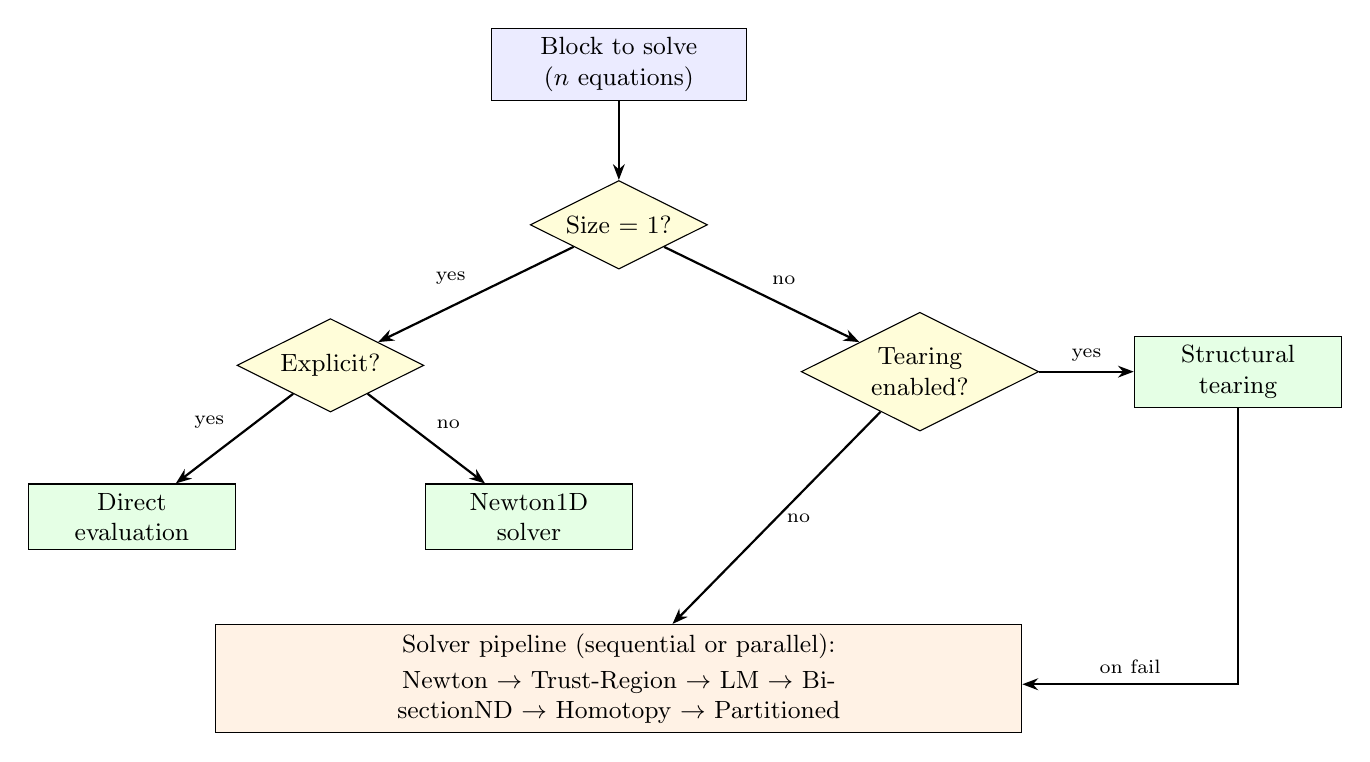
\begin{tikzpicture}[
    node distance=0.8cm,
    block/.style={rectangle, draw, fill=blue!8, text width=3cm, minimum height=0.7cm, align=center, font=\small},
    decision/.style={diamond, draw, fill=yellow!15, text width=1.6cm, minimum height=0.5cm, align=center, font=\small, inner sep=1pt, aspect=2},
    solver/.style={rectangle, draw, fill=green!10, text width=2.4cm, minimum height=0.7cm, align=center, font=\small},
    pipelinebox/.style={rectangle, draw, fill=orange!10, text width=10cm, minimum height=1cm, align=center, font=\small},
    arrow/.style={-{Stealth[length=2mm]}, thick},
]
% Row 1: Start
\node[block] (start) {Block to solve\\($n$ equations)};

% Row 2: Size check
\node[decision, below=1cm of start] (size1) {Size $= 1$?};
\draw[arrow] (start) -- (size1);

% Left branch: size 1
\node[decision, below left=1.2cm and 2.5cm of size1] (explicit) {Explicit?};
\draw[arrow] (size1) -- node[above left, font=\scriptsize]{yes} (explicit);

\node[solver, below left=1.2cm and 0.6cm of explicit] (direct) {Direct\\evaluation};
\draw[arrow] (explicit) -- node[above left, font=\scriptsize]{yes} (direct);

\node[solver, below right=1.2cm and 0.6cm of explicit] (n1d) {Newton1D\\solver};
\draw[arrow] (explicit) -- node[above right, font=\scriptsize]{no} (n1d);

% Right branch: size > 1
\node[decision, below right=1.2cm and 2.5cm of size1] (tearing) {Tearing\\enabled?};
\draw[arrow] (size1) -- node[above right, font=\scriptsize]{no} (tearing);

\node[solver, right=1.2cm of tearing] (tear) {Structural\\tearing};
\draw[arrow] (tearing) -- node[above, font=\scriptsize]{yes} (tear);

% Bottom: Pipeline — positioned below everything
\node[pipelinebox, below=4.5cm of size1] (pipeline) {%
Solver pipeline (sequential or parallel):\\[2pt]
Newton $\rightarrow$ Trust-Region $\rightarrow$ LM $\rightarrow$ BisectionND $\rightarrow$ Homotopy $\rightarrow$ Partitioned};
\draw[arrow] (tearing) -- node[right, font=\scriptsize]{no} (pipeline);
\draw[arrow] (tear) |- ([yshift=-2pt]pipeline.east) node[near end, above, font=\scriptsize]{on fail};
\end{tikzpicture}
\caption{Solver pipeline strategy for each equation block. The pipeline supports sequential (try in order) and parallel (first-to-converge wins) execution modes.}
\label{fig:pipeline}
\end{figure}

% ===================================================================
\section{Automatic Differentiation}
\label{sec:ad}
% ===================================================================

CoolSolve computes exact Jacobian matrices using forward-mode automatic differentiation (AD) rather than finite differences. Each expression is evaluated as a dual number $(v, \mathbf{g})$ where $v$ is the scalar value and $\mathbf{g} \in \mathbb{R}^n$ is the gradient vector (partial derivatives with respect to all $n$ block unknowns).

The propagation rules follow the chain rule:
\begin{align}
    (x + y).g &= x.g + y.g \\
    (x \cdot y).g &= x.g \cdot y.v + y.g \cdot x.v \\
    (x^n).g &= n \, x^{n-1} \cdot x.g \\
    \sin(x).g &= \cos(x.v) \cdot x.g
\end{align}
and similarly for all supported operations ($+, -, \times, /, \hat{\ }$, \texttt{sin}, \texttt{cos}, \texttt{exp}, \texttt{log}, \texttt{sqrt}, etc.).

This approach provides exact analytical derivatives (to machine precision), avoids the accuracy issues of finite differences, and eliminates the need for $2n$ additional function evaluations per Jacobian row that central differences would require.

For CoolProp property evaluations, CoolSolve uses CoolProp's \texttt{first\_partial\_deriv()} function for analytical thermodynamic derivatives, with a forward-FD consistency check. This is detailed in Section~\ref{sec:coolprop}.

% ===================================================================
\section{CoolProp Integration}
\label{sec:coolprop}
% ===================================================================

CoolProp \cite{Bell2014} is an open-source library that provides thermophysical properties for over 120 pure and pseudo-pure fluids, as well as mixtures and incompressible fluids. CoolSolve integrates CoolProp at a deep level to achieve both accuracy and computational performance.

\subsection{Thermodynamic Property Calls}

When the parser encounters a thermodynamic function call such as \texttt{enthalpy(Water, T=373, P=101325)}, the evaluator:
\begin{enumerate}
    \item Identifies the fluid name (\texttt{Water}), the output property (enthalpy), and the input pair (temperature and pressure).
    \item Maps the input pair to the appropriate CoolProp input specification (e.g., \texttt{PT\_INPUTS}).
    \item Calls CoolProp to compute the property value.
    \item If the Jacobian is needed, computes the derivatives of the output property with respect to each input that is a block unknown.
\end{enumerate}

CoolSolve automatically handles the temperature convention: the EES language uses Celsius, while CoolProp uses Kelvin. The conversion is applied transparently during evaluation.

\subsection{Low-Level API and Caching}

For performance, CoolSolve uses CoolProp's low-level \texttt{AbstractState} API rather than the high-level \texttt{PropsSI} function. The \texttt{AbstractState} API avoids repeated string parsing and fluid lookup by caching initialized fluid objects. CoolSolve maintains a thread-local cache that maps \texttt{(backend, fluid)} pairs to reusable \texttt{AbstractState} instances:

\begin{itemize}
    \item \textbf{Thread-local storage} ensures thread safety in parallel mode without mutex contention.
    \item \textbf{Automatic fallback}: if the \texttt{AbstractState} API throws (e.g., for unsupported fluid types), CoolSolve falls back to \texttt{PropsSI}.
    \item \textbf{Configurable backend}: supports \texttt{HEOS} (default), \texttt{TTSE\&HEOS} (tabular interpolation), and \texttt{BICUBIC\&HEOS}.
\end{itemize}

\subsection{Analytical Derivatives with Consistency Check}

CoolProp's \texttt{first\_partial\_deriv()} function provides analytical thermodynamic derivatives from the equation of state. However, these derivatives can be inaccurate near phase boundaries for pseudo-pure fluids (e.g., Air $\approx$ N$_2$/O$_2$/Ar mixture). CoolSolve implements a \textbf{forward-FD consistency check}:
\begin{enumerate}
    \item Compute analytical derivatives via \texttt{first\_partial\_deriv()} (zero extra state evaluations).
    \item Compute forward-FD derivatives (two extra \texttt{update()} calls per property).
    \item If the analytical and FD values agree within 5\%: use the analytical derivatives.
    \item If they disagree: use the FD values (indicating a phase-boundary region).
    \item If \texttt{first\_partial\_deriv()} throws: fall back to central FD.
\end{enumerate}

This hybrid approach provides exact derivatives in the vast majority of cases while automatically detecting and correcting the rare situations where analytical derivatives are unreliable. The consistency check adds modest overhead (2 extra \texttt{update()} calls per property) but prevents corrupted Jacobians that would cause solver failure.

\subsection{Residual-Only Evaluation Mode}

During line search backtracking, only the residual $\mathbf{F}(\mathbf{x})$ is needed---not the Jacobian. CoolSolve implements a \textbf{residual-only evaluation mode} that skips all derivative computation (no \texttt{first\_partial\_deriv()}, no FD perturbations, no gradient propagation in the AD engine). This reduces the cost of each line search evaluation to a single \texttt{AbstractState::update()} call per property, providing a 3--5$\times$ speedup during backtracking.

% ===================================================================
\section{Web-Based Graphical User Interface}
\label{sec:gui}
% ===================================================================

CoolSolve includes an optional web-based GUI that provides a complete modeling environment accessible from any web browser (Fig.~\ref{fig:gui}). The GUI is implemented as a React/TypeScript single-page application communicating with the CoolSolve C++ backend via a REST API.

\subsection{Architecture}

The GUI is served by an embedded HTTP server (cpp-httplib) inside the CoolSolve binary. Running \texttt{coolsolve --gui} starts the server and opens the user's default browser. The same compiled binary contains both the CLI solver and the embedded web server with all frontend assets, requiring \textbf{zero external runtime dependencies} (no Node.js, no Python, no Java).

The same GUI works in two deployment scenarios:
\begin{itemize}
    \item \textbf{Local}: the user runs the binary on their machine, and the browser connects to \texttt{localhost}.
    \item \textbf{Online}: the binary runs behind a reverse proxy (e.g., Apache or Nginx) on a server, enabling shared access through a URL (e.g., \url{https://coolsolve.squoilin.eu}).
\end{itemize}

\subsection{Features}

The GUI provides:
\begin{itemize}
    \item A \textbf{code editor} (Monaco Editor, the same engine used in VS Code) with EES syntax highlighting, real-time parse error markers, comment toggling, and find/replace.
    \item \textbf{Real-time solving} with progress streaming via Server-Sent Events (SSE): the user sees each block being solved in real time.
    \item A \textbf{variable table} showing solved values, initial guesses (editable), and unit annotations. An array table provides a spreadsheet view for indexed variables.
    \item A \textbf{configuration editor} for all solver options, with preset pipelines and individual parameter tuning.
    \item \textbf{Debug mode}: generates a comprehensive set of diagnostic files (solver traces, block-by-block residuals, incidence matrices, equation listings) visible in the browser.
    \item \textbf{Parametric studies}: 1D and 2D sweeps over imposed variables, with warm-starting (each grid point uses the nearest previously-converged solution as initial guesses).
    \item \textbf{Interactive thermodynamic diagrams}: T-s, P-h, h-s, and T-h diagrams with saturation dome and solved state point overlay.
    \item \textbf{ZIP bundle import/export}: models can be saved and shared as ZIP archives containing the source code, initial guesses, solution, and solver configuration.
\end{itemize}

\begin{figure*}[htbp]
\centering

\includegraphics[width=\textwidth]{coolsolve_gui.png}
\caption{Screenshot of the CoolSolve web-based graphical user interface showing the code editor, variable table, and solver output.}
\label{fig:gui}
\end{figure*}

% ===================================================================
\section{Validation and Results}
\label{sec:validation}
% ===================================================================

CoolSolve is validated on a comprehensive test suite of 40 thermodynamic models covering a wide range of energy conversion systems. The example models include:

\begin{itemize}
    \item \textbf{Rankine and organic Rankine cycles}: simple and complex ORC models with various working fluids (R245fa, CO$_2$, R134a), including recuperated cycles, extraction turbines, and supercritical configurations \cite{Quoilin2011, Quoilin2013}.
    \item \textbf{Refrigeration cycles}: simple vapor-compression, multi-stage, and compound cycles.
    \item \textbf{Heat pumps}: single- and multi-source heat pump models \cite{Lemort2009}.
    \item \textbf{Compressors}: scroll, piston, screw, centrifugal, and turbo-compressor models.
    \item \textbf{Heat exchangers}: condensers (wet, dry, 3-zone moving-boundary), evaporators, cooling towers, cooling coils \cite{Desideri2014}.
    \item \textbf{Combustion engines}: internal combustion engine models with ideal-gas and real-fluid properties.
    \item \textbf{Humid air processes}: psychrometric calculations using humid air properties.
\end{itemize}

Model complexity ranges from 30 equations (simple Rankine cycle, all blocks of size 1) to 173 equations with algebraic loops of up to 63 coupled unknowns.

\subsection{Solution Verification}

After a successful solve, CoolSolve independently re-evaluates every equation using the proposed solution and checks that $|\text{LHS} - \text{RHS}|/\max(|\text{LHS}|, 1) < 0.1\%$. This \emph{solution verification} step catches numerical drift, structural bugs, and procedure output inconsistencies that the solver's own convergence check may miss.

\subsection{Robustness Results}

Table~\ref{tab:robustness} summarizes the solver robustness results across different configurations. Of the 40 models, 39 are parseable (one requires an unsupported \texttt{MODULE} construct), and 38 are solvable in at least one configuration.

\begin{table}[htbp]
\centering
\caption{Solver robustness results across configurations. ``With initials'' means initial guesses are provided; ``No initials'' means all unknowns start at the default value.}
\label{tab:robustness}
\begin{tabular}{@{}lccc@{}}
\toprule
\textbf{Configuration} & \textbf{With initials} & \textbf{No initials} \\
\midrule
Default pipeline (6 solvers) & 36/39 (92.3\%) & 26/38 (68.4\%) \\
Newton only                   & 32/39 (82.1\%) & 19/38 (50.0\%) \\
Trust-Region only             & 34/39 (87.2\%) & 18/38 (47.4\%) \\
Levenberg-Marquardt only      & 28/39 (71.8\%) & 15/38 (39.5\%) \\
BisectionND only              & 15/39 (38.5\%) & 13/38 (34.2\%) \\
Homotopy only                 & 32/39 (82.1\%) & 22/38 (57.9\%) \\
Default + Tearing             & 36/39 (92.3\%) & 26/38 (68.4\%) \\
Default + Symbolic Reduction  & 36/39 (92.3\%) & 26/38 (68.4\%) \\
\bottomrule
\end{tabular}
\end{table}

The results demonstrate that:
\begin{enumerate}
    \item The multi-solver pipeline significantly outperforms any individual solver. The 92.3\% success rate of the full pipeline compares to 82.1\% for Newton alone and 71.8\% for LM alone.
    \item Homotopy continuation is the most robust individual solver for problems without initial guesses (57.9\%), confirming its value as a global convergence method.
    \item The ``no initials'' scenario (all variables start at 1.0) is much harder, dropping from 92.3\% to 68.4\%. This underscores the importance of good initial guesses for thermodynamic models, but also shows that the pipeline can converge two-thirds of models even with no initialization.
    \item BisectionND is effective only for small blocks but provides unique value as the only derivative-free method.
\end{enumerate}

\subsection{Solve Time Performance}

Table~\ref{tab:timing} presents solve times for representative models.

\begin{table}[htbp]
\centering
\caption{Solve time for representative thermodynamic models (Release build, default pipeline with initials).}
\label{tab:timing}
\begin{tabular}{@{}lcccr@{}}
\toprule
\textbf{Model} & \textbf{Eqs} & \textbf{Blocks} & \textbf{Largest block} & \textbf{Time (s)} \\
\midrule
Rankine cycle (simple)       & 30  & 30  & 1   & $<$0.01 \\
Refrigeration (R134a)        & 30  & 30  & 1   & $<$0.01 \\
ORC simple (R245fa)          & 172 & 150 & 8   & 0.03 \\
ORC with CO$_2$              & 139 & 112 & 28  & 0.02 \\
Heat pump (R22)              & ---  & 17  & 39  & 0.01 \\
Scroll compressor            & 99  & 66  & 34  & 0.09 \\
Condenser 3-zone             & 111 & 50  & 62  & 0.03 \\
Heat pump (Zorlu)            & 126 & 64  & 63  & 0.03 \\
Cooling tower                & --- & 14  & 11  & 4.87 \\
\bottomrule
\end{tabular}
\end{table}

Most models solve in under 100~ms. The \texttt{cooling\_tower2} model is an outlier at 4.87~s due to stiff CoolProp evaluations near the wet-bulb temperature, requiring the homotopy solver for convergence.

\subsection{Comparison with EES}

CoolSolve provides a comparison mode (\texttt{-c} flag) that validates its structural analysis against EES output. For all models tested, CoolSolve produces the same variable-equation matching and block decomposition as EES, confirming structural correctness. Numerical solutions are validated to 1\% tolerance against EES reference solutions where available.

% ===================================================================
\section{Software Availability and Deployment}
\label{sec:availability}
% ===================================================================

CoolSolve is released under the MIT open-source license. All source code, example models, documentation, and test suites are publicly available on GitHub \cite{CoolSolve2026}:
\begin{center}
    \url{https://github.com/squoilin/coolsolve}
\end{center}

The software is cross-platform and has been tested on Linux (Ubuntu 22.04/24.04), macOS, and Windows. It requires only a C++17 compiler and CMake 3.14+; all library dependencies (CoolProp, Eigen, cpp-peglib, nlohmann/json, Catch2) are automatically downloaded and compiled via CMake FetchContent.

For users who do not wish to compile the software, a publicly accessible online instance is available at:
\begin{center}
    \url{https://coolsolve.squoilin.eu}
\end{center}
This online deployment uses the same binary and GUI described in Section~\ref{sec:gui}, served behind an Apache reverse proxy with session-based sandboxing.

% ===================================================================
\section{Conclusion}
\label{sec:conclusion}
% ===================================================================

This paper has presented CoolSolve, an open-source equation solver for thermodynamic system modeling. By implementing a language compatible with the widely-used EES syntax and integrating the open-source CoolProp thermodynamic property library, CoolSolve lowers the barrier to building, sharing, and reproducing thermodynamic models.

The key innovations compared to existing tools are:
\begin{enumerate}
    \item A \textbf{configurable multi-solver pipeline} with six complementary algorithms, including Newton with non-monotone line search, Trust-Region Dogleg, Levenberg-Marquardt with geodesic acceleration, N-dimensional bisection, homotopy continuation, and partitioned block updates. The pipeline supports both sequential and parallel execution, achieving a 92.3\% solve rate on 39 thermodynamic models with initial guesses.
    \item \textbf{Structural analysis and symbolic reduction}: Hopcroft-Karp matching and Tarjan's SCC decomposition automatically partition equation systems into solvable blocks. Optional symbolic preprocessing with post-reduction re-decomposition further reduces block sizes.
    \item \textbf{Deep CoolProp integration}: low-level API with thread-local caching, analytical derivatives with consistency check, and residual-only evaluation mode for efficient line search.
    \item A \textbf{web-based GUI} enabling browser-based modeling with real-time solving, parametric studies, and interactive thermodynamic diagrams, deployable both locally and online.
    \item \textbf{Full open-source availability}: all code, models, and documentation are publicly accessible, supporting the growing call for transparency and reproducibility in energy research \cite{Pfenninger2017}.
\end{enumerate}

Future work includes extending the parser to cover the full EES language (including \texttt{MODULE} support, lookup tables, and string processing), improving solver robustness for the ``no initial guess'' scenario, and developing a library of validated component models for common HVAC\&R and power cycle equipment.

% ===================================================================
% Acknowledgments
% ===================================================================

% ===================================================================
% References
% ===================================================================
\section*{Declaration of Competing Interest}
The author declares that he has no known competing financial interests or personal relationships that could have appeared to influence the work reported in this paper.

\section*{CRediT authorship contribution statement}
\textbf{Sylvain Quoilin}: Conceptualization, Methodology, Software, Validation, Writing -- original draft, Writing -- review \& editing.

\section*{Data availability}
All source code, example models, and data are available on GitHub at \url{https://github.com/squoilin/coolsolve} (MIT license). An online instance is accessible at \url{https://coolsolve.squoilin.eu}.

\bibliographystyle{elsarticle-num}
\bibliography{references}

\end{document}
